\label{sec:Zjets}
The requirement of high \met in the final state reduces the available number of events in the $Z$+jet Monte Carlo sample
to a level where it is impossible to construct a smooth template.  To overcome this problem, we construct $Z$+jet template 
from events with a lower \met requirement. The range of \met used to construct the template is $m_{H}$
dependent and provided in 
Table~\ref{tab:interMET}.  
It should be noted that such a solution is possible because \met is not directly used in the calculation
of the event probabilities; instead, it is inferred from the transverse momenta of charged leptons and the system boost.
To verify that there is no large bias due to a LR shape dependence on \met, we compare shapes of the likelihood distribution
in $Z$+jet Monte Carlo events for three different \met regions,  shown in Fig.~\ref{fig:LRshapeMET}.
The shapes are found to be consistent with each other within statistical uncertainties.
The residual difference between the nominal LR shape and the one obtained from the lower \met region is assigned 
as a systematic uncertainty.    

To ensure that Monte Carlo adequately describes the kinematic features of $Z$+jet events in data, we compare LR shapes
in data to MC in the region $40<\met<50$ GeV, which is dominated by $Z$+jet events at the $> 90\%$ level
and does not suffer from low statistics. 
The comparison shown in Fig~\ref{fig:LRshapeMETDataMC} reveals good agreement between data and MC.

\begin{table}[!hbtp]
\begin{center}
\begin{tabular}{c c}
\hline\hline
 $m_H$ (\GeVcc) & $\met$ cut range (GeV)\\
\hline
\hline
 250 & 50--60 \\
 300 & 50--70 \\
 350 & 50--80 \\
 400 & 50--80 \\
 500 & 50--100\\
 600 & 50--120\\
\hline
\end{tabular}
\caption{Summary of the \met ranges used for constructing the $Z$+jet likelihood ratio.}
\label{tab:interMET}
\end{center}
\end{table}

\begin{figure}[!hbtp]                                                                                         
\centering    
\subfigure[]{                                                                                                 
\centering                                                                                                    
\label{subfig:lr_met250}                                                                            
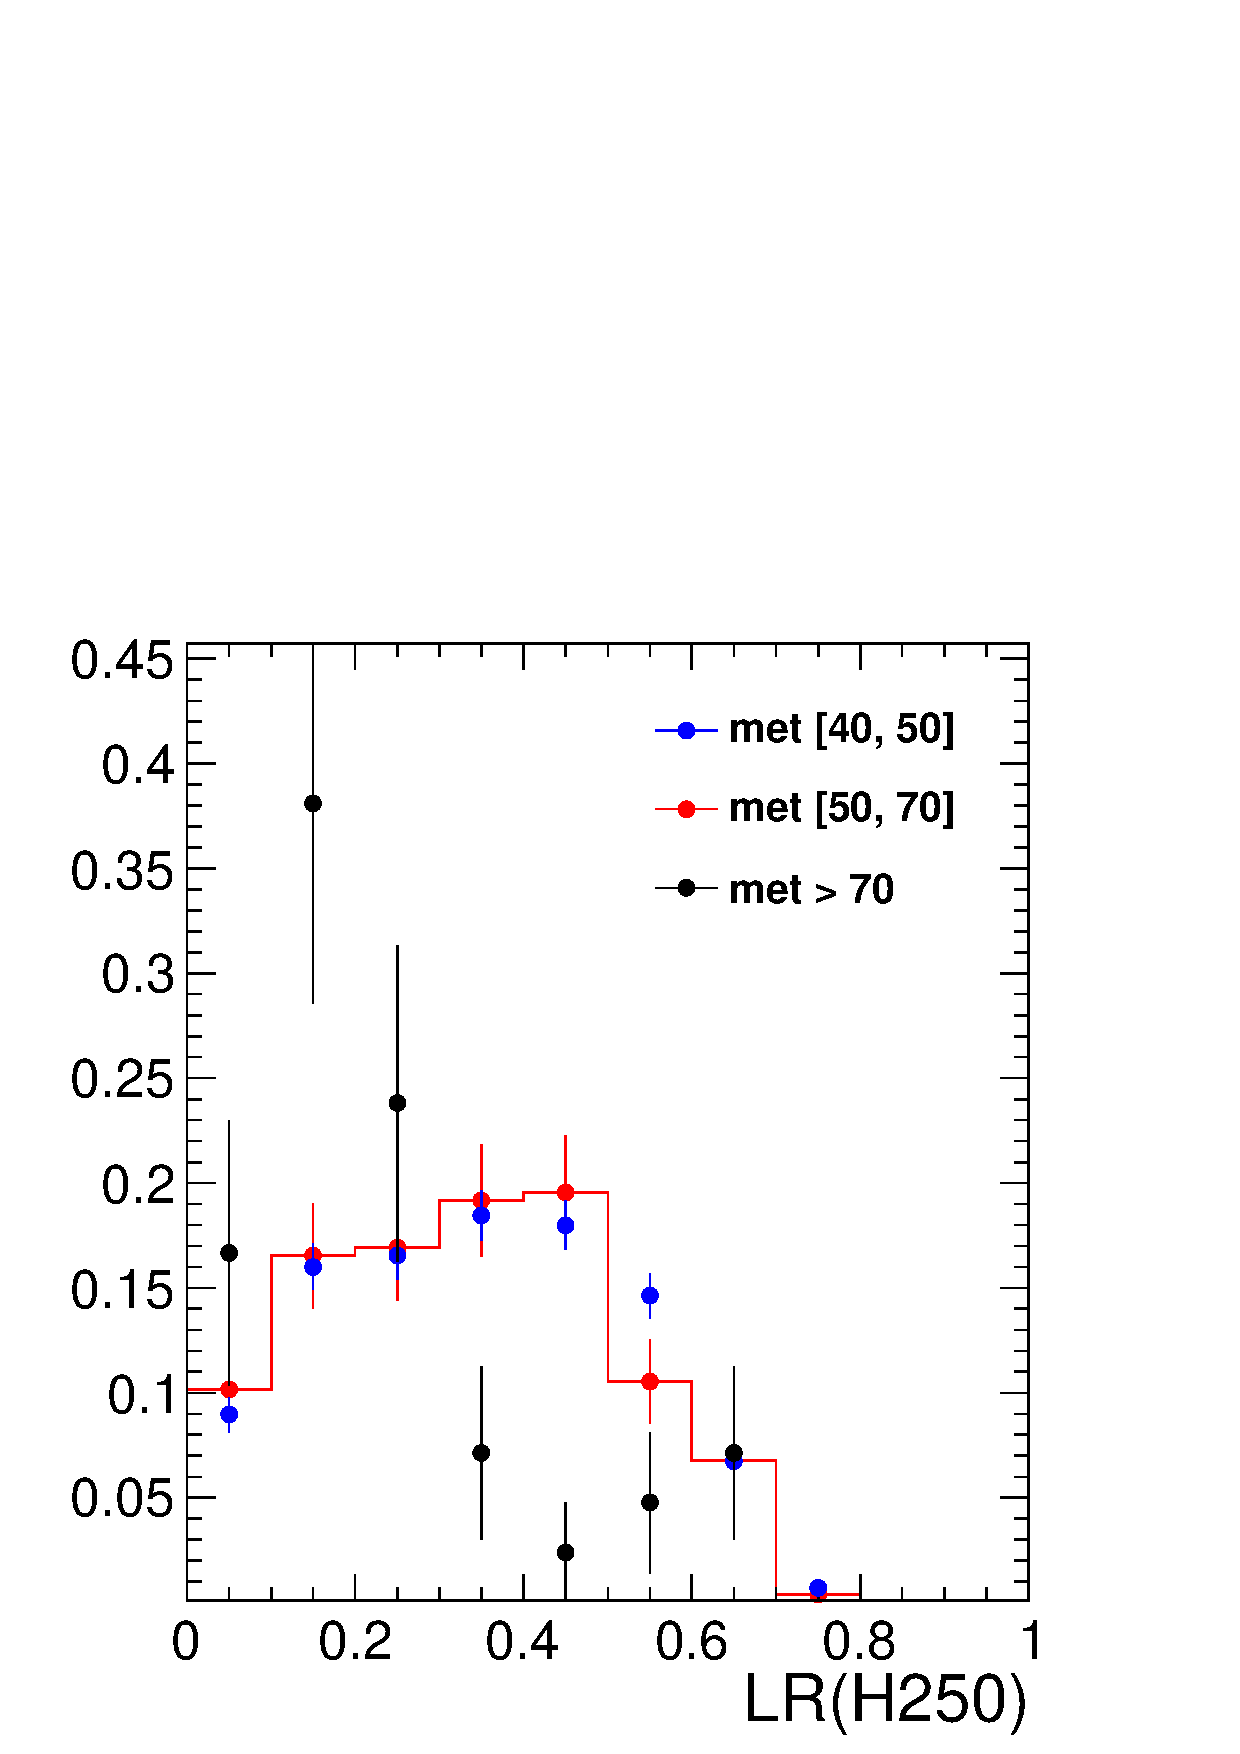
\includegraphics[width=.30\textwidth]{figures/Zee_LR_mH250_lin.png}         
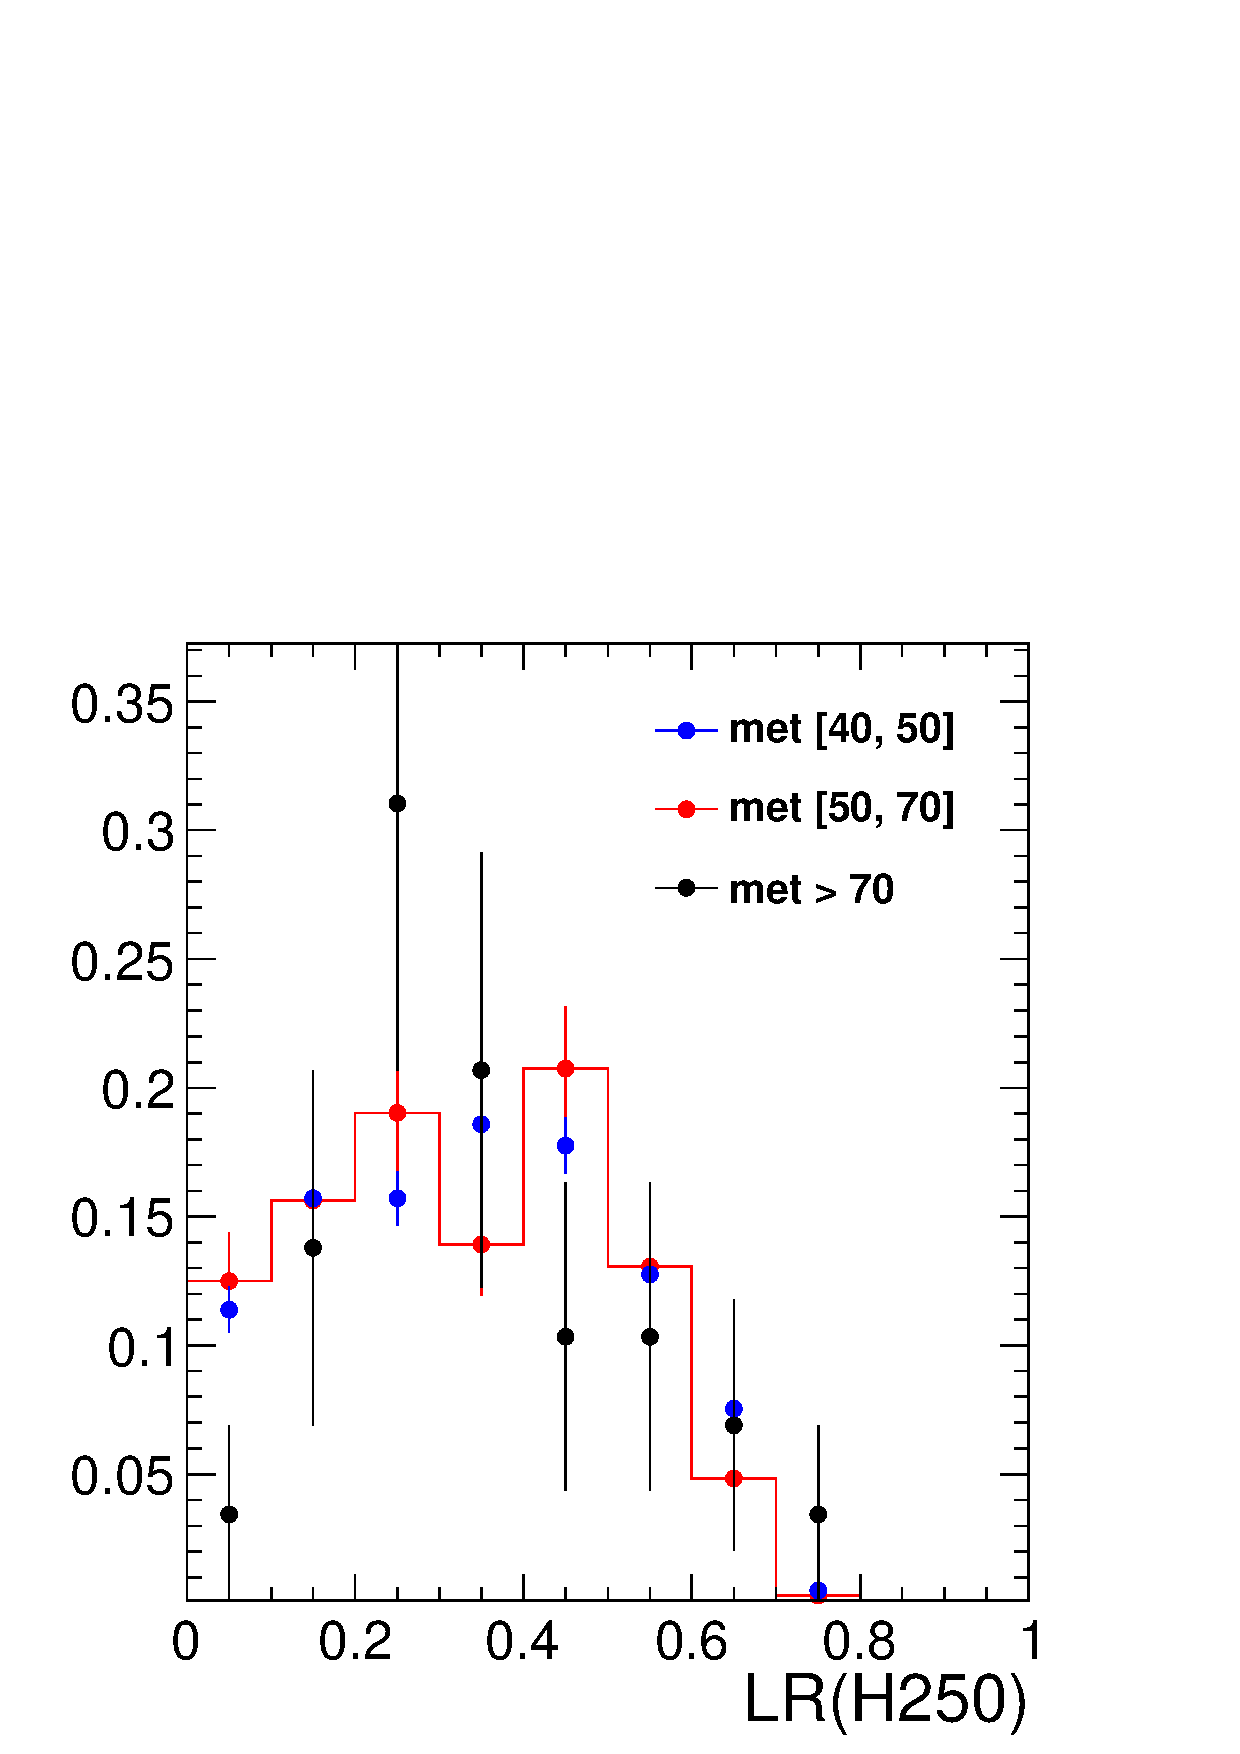
\includegraphics[width=.30\textwidth]{figures/Zmm_LR_mH250_lin.png}} 
\subfigure[]{                                                                                                 
\centering                                                                                                    
\label{subfig:lr_met300}                                                                            
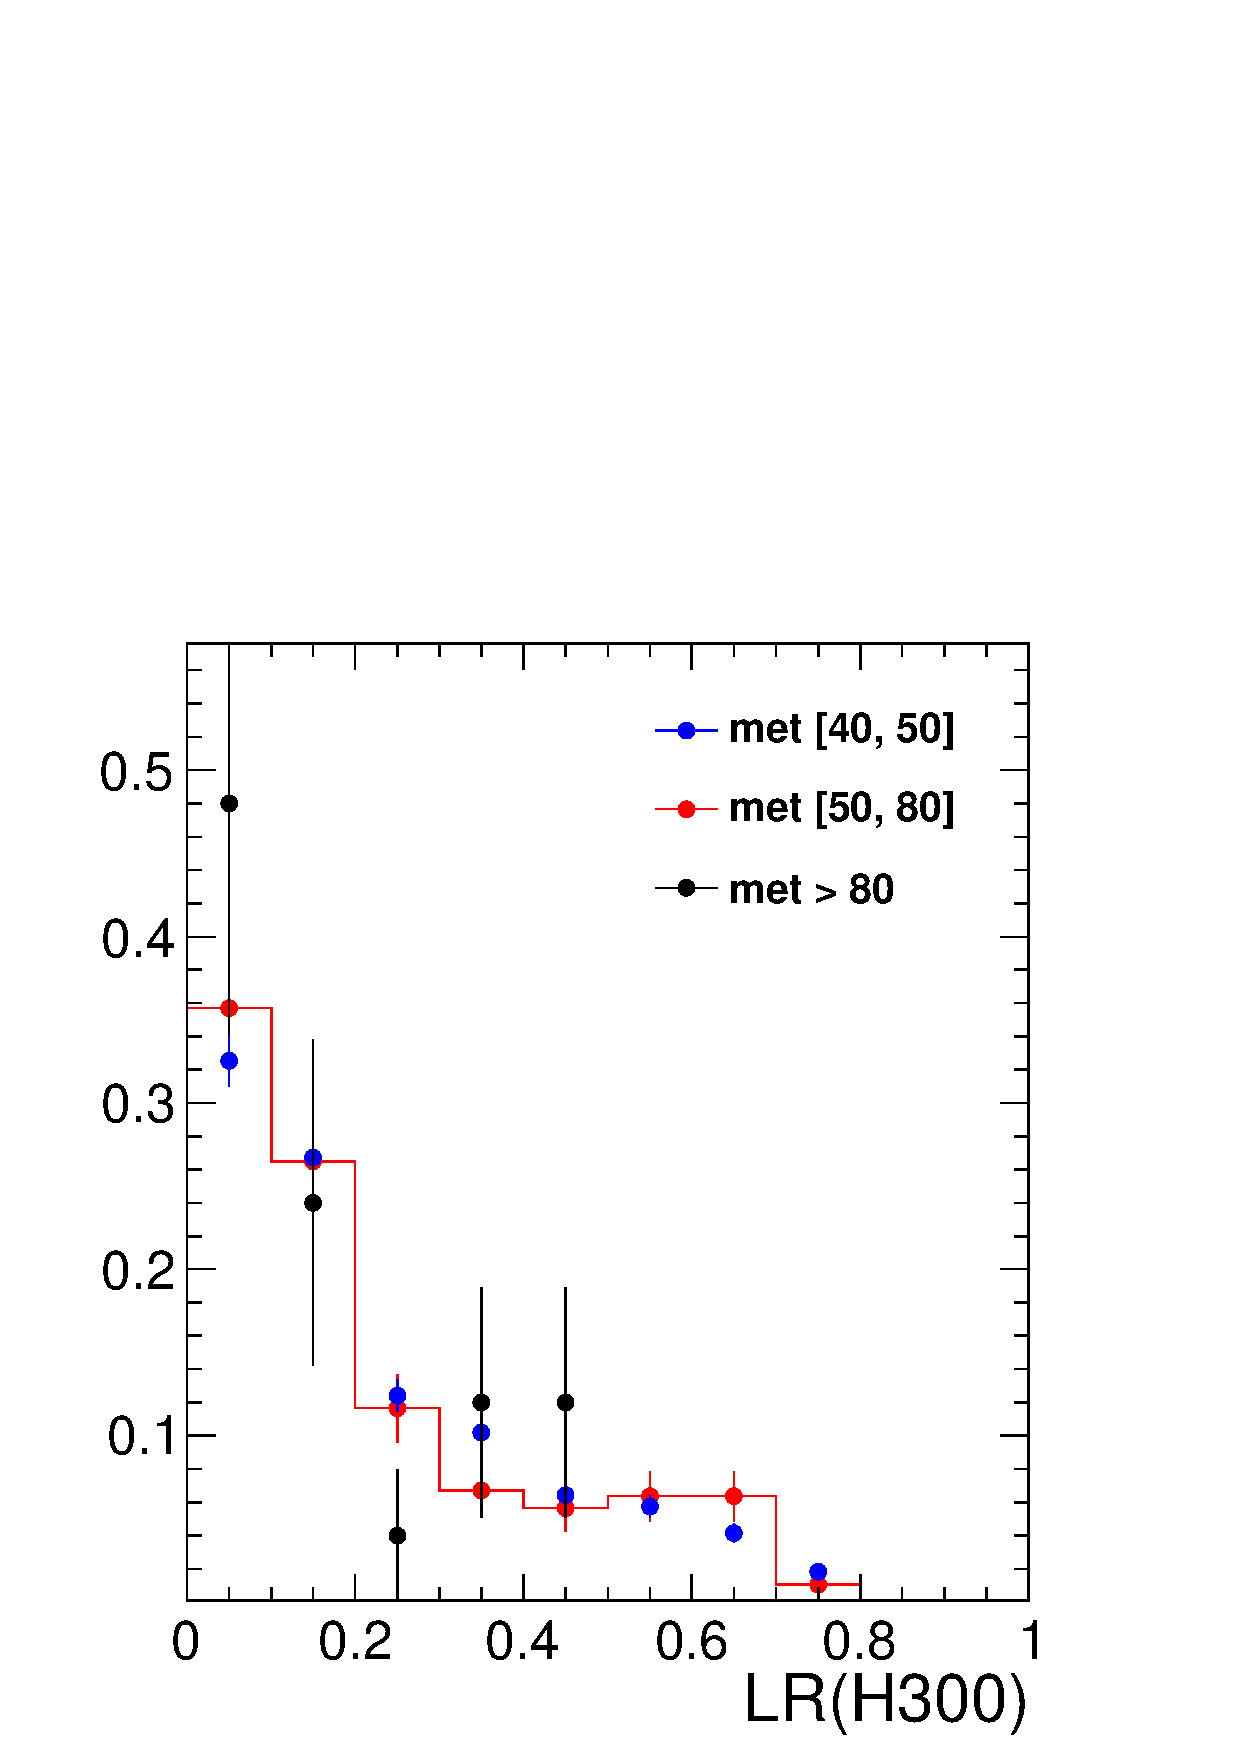
\includegraphics[width=.30\textwidth]{figures/Zee_LR_mH300_lin.png}         
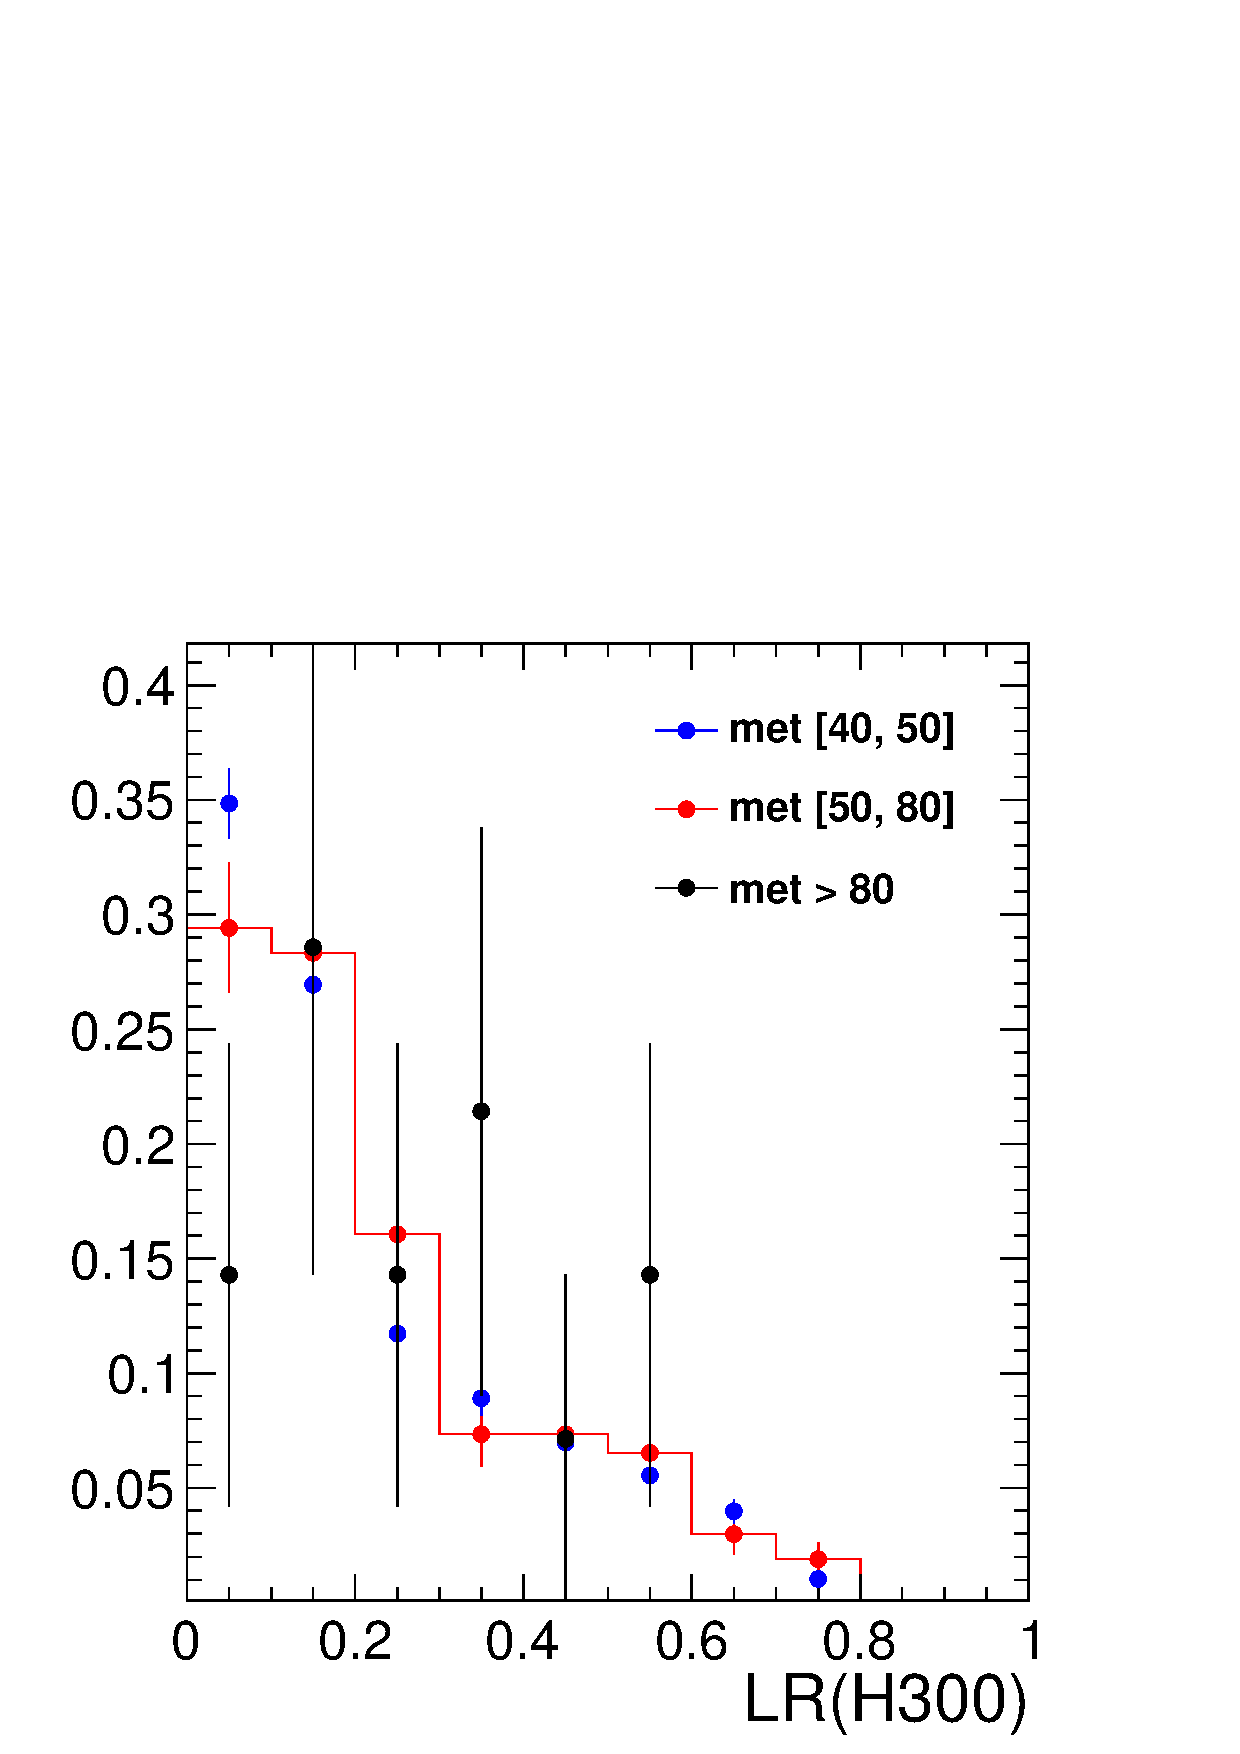
\includegraphics[width=.30\textwidth]{figures/Zmm_LR_mH300_lin.png}}                                            
\subfigure[]{                                                                                                 
\centering                                                                                                    
\label{subfig:lr_met350}                                                                            
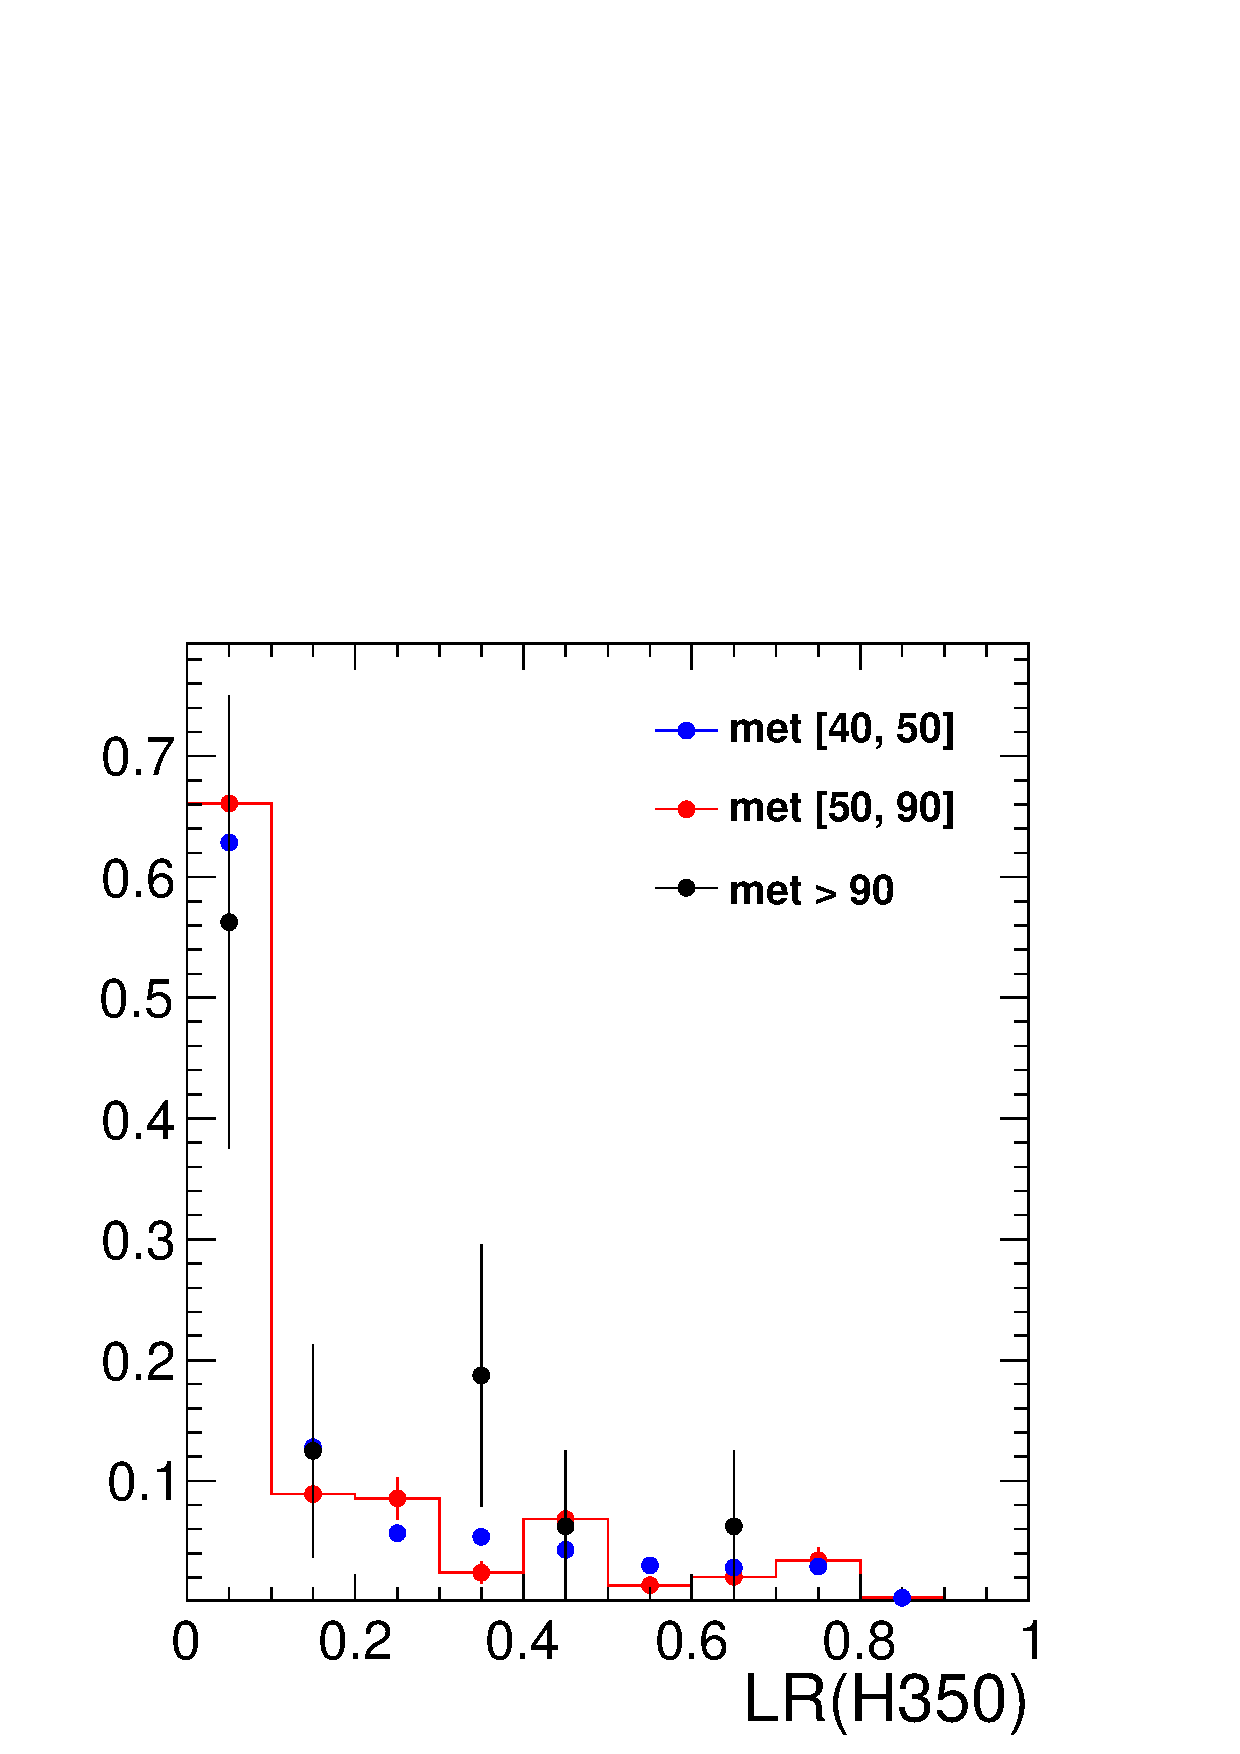
\includegraphics[width=.30\textwidth]{figures/Zee_LR_mH350_lin.png}         
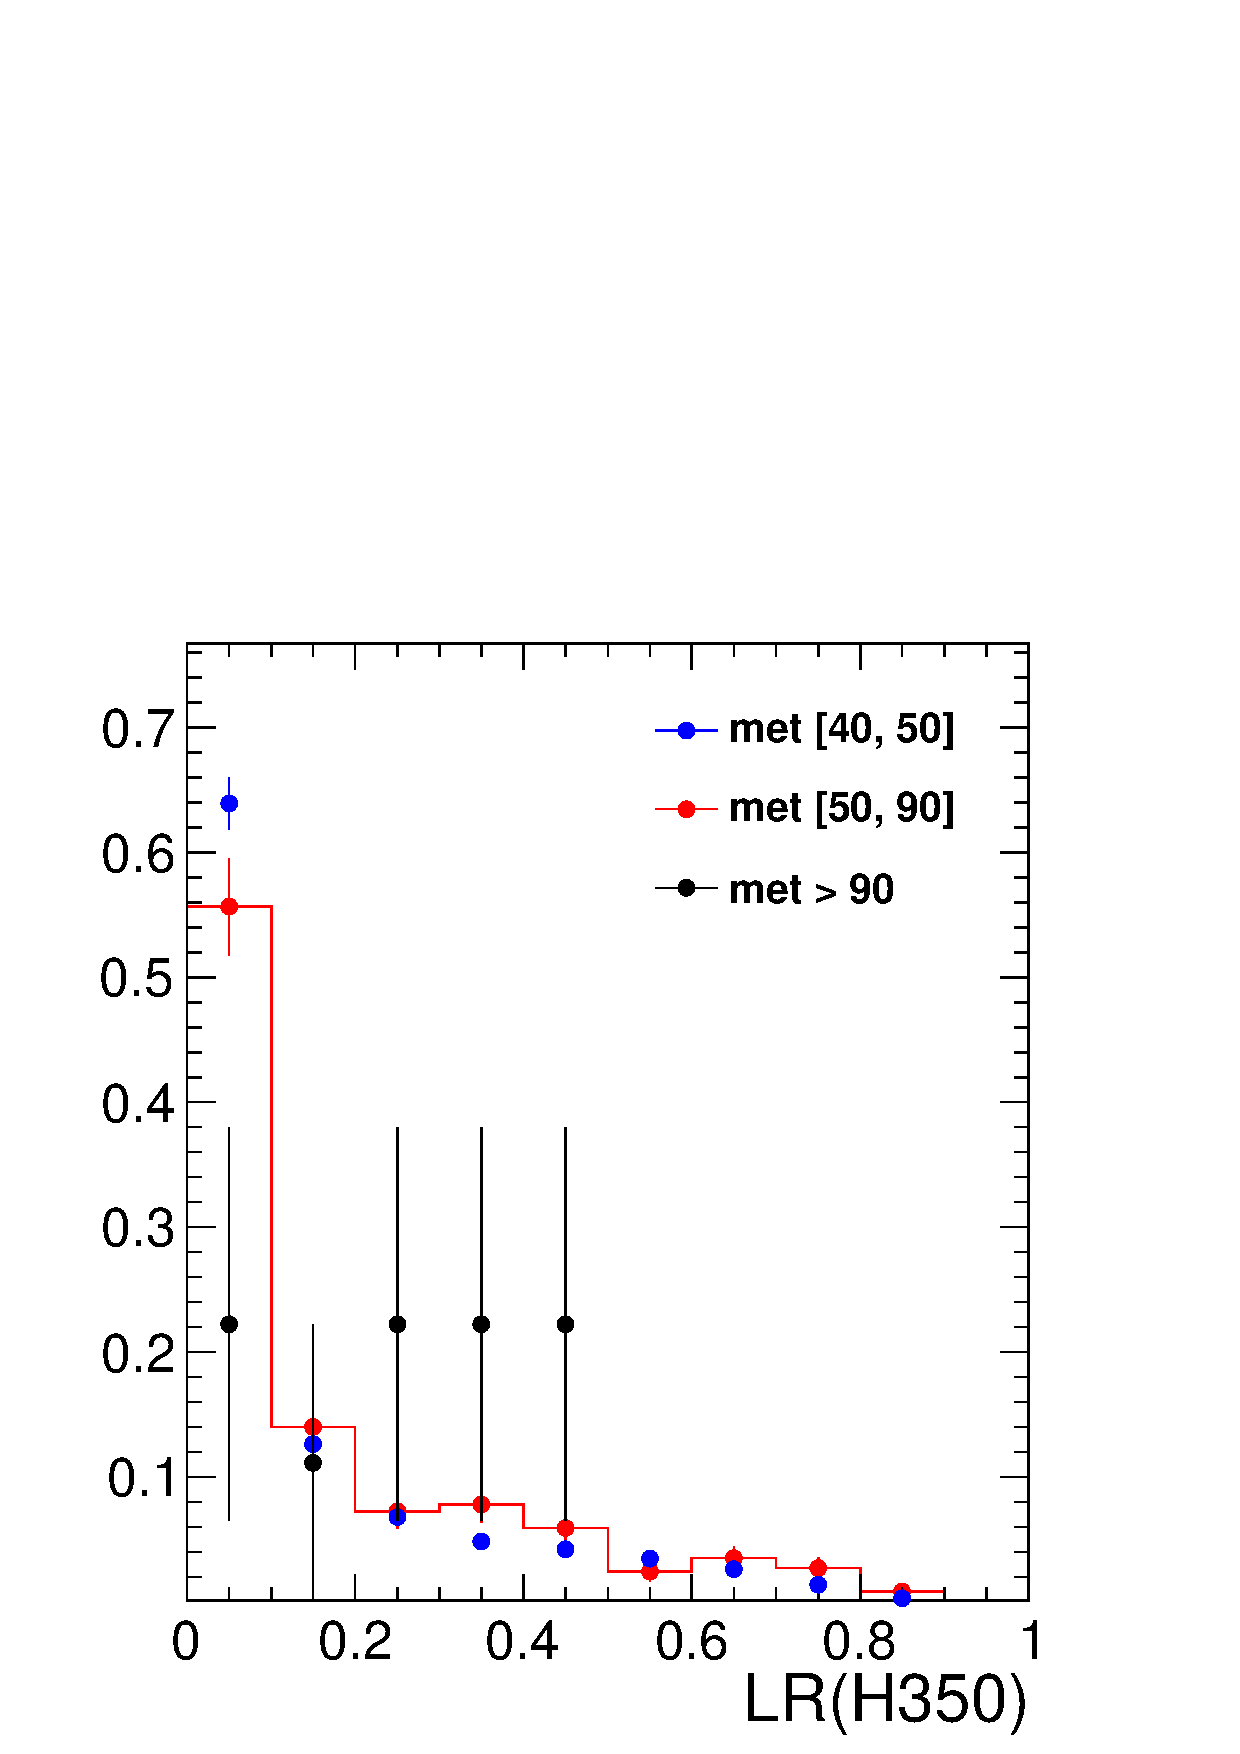
\includegraphics[width=.30\textwidth]{figures/Zmm_LR_mH350_lin.png}}
\subfigure[]{                                                                                                 
\centering                                                                                                    
\label{subfig:lr_met400}                                                                            
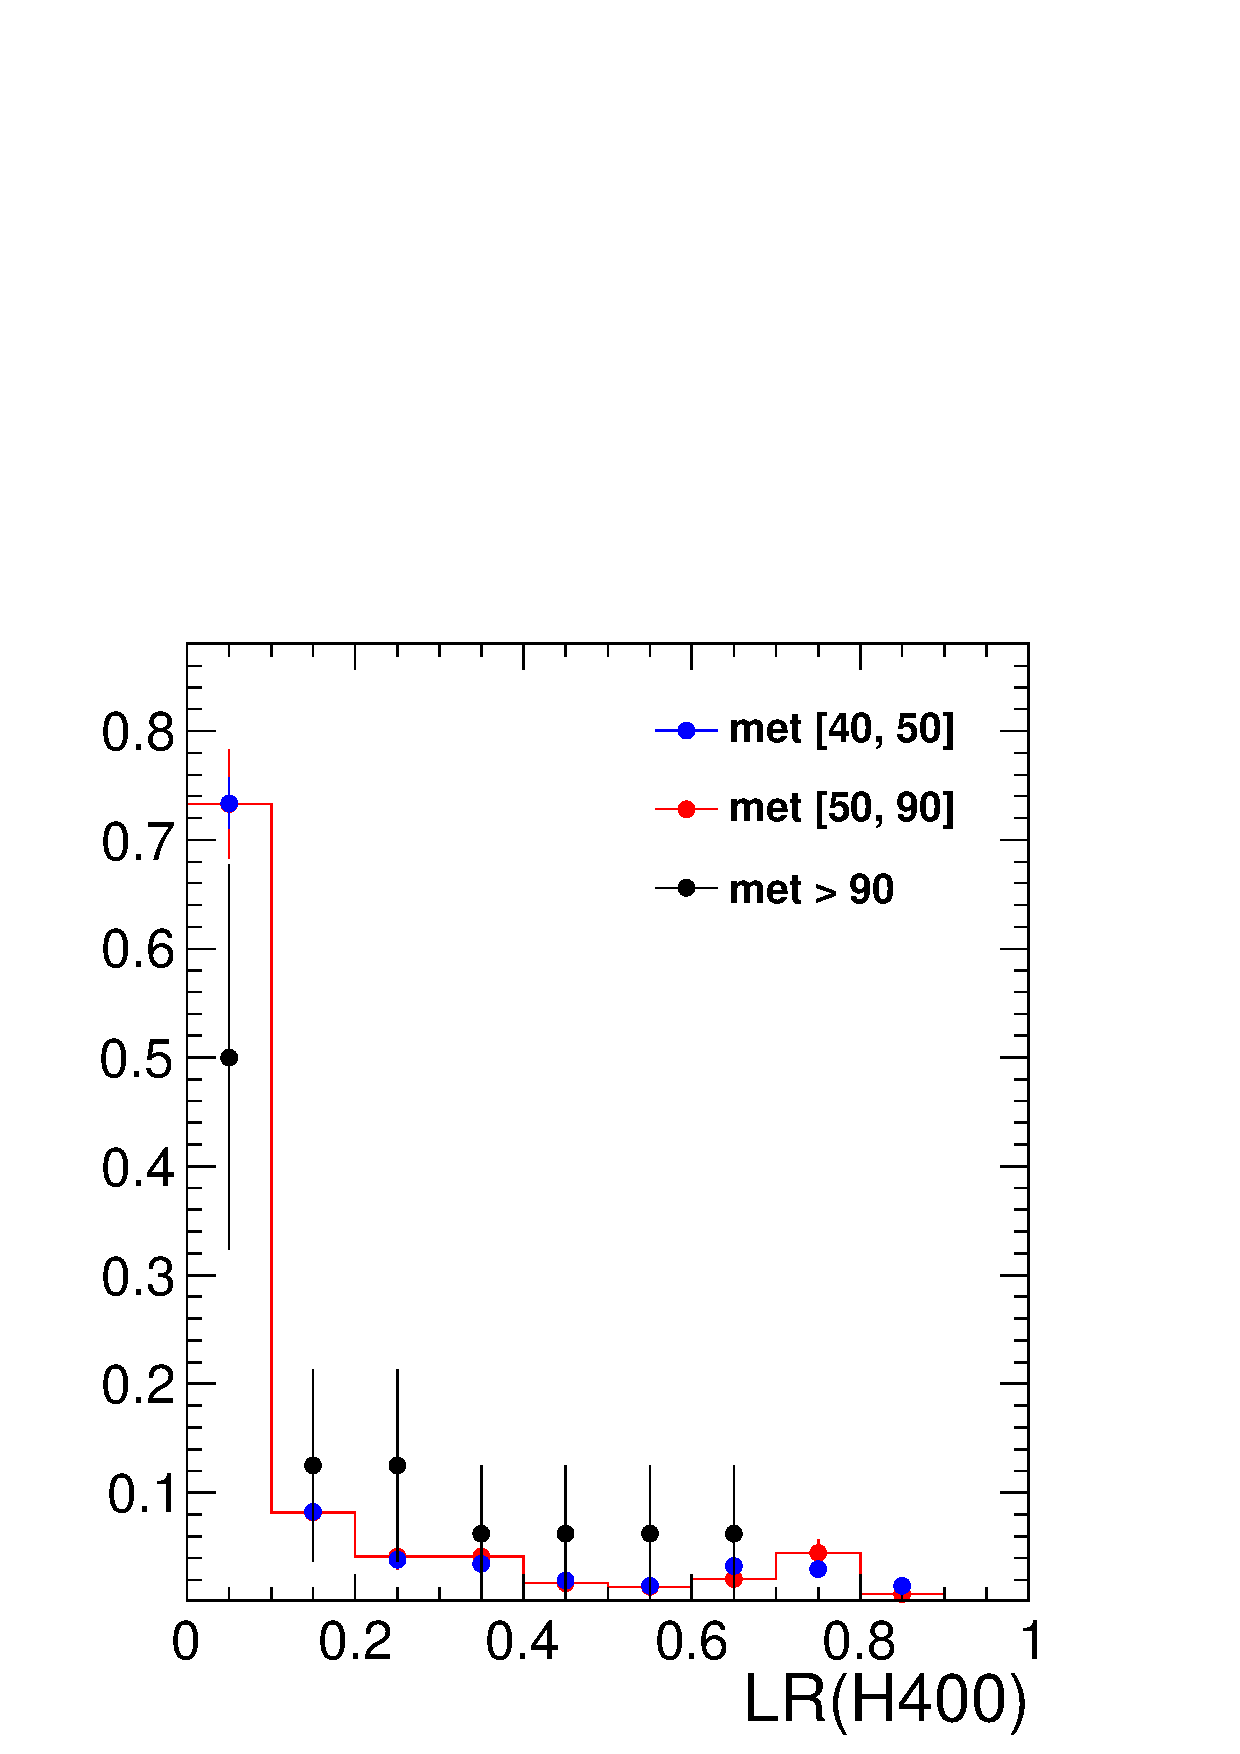
\includegraphics[width=.30\textwidth]{figures/Zee_LR_mH400_lin.png}         
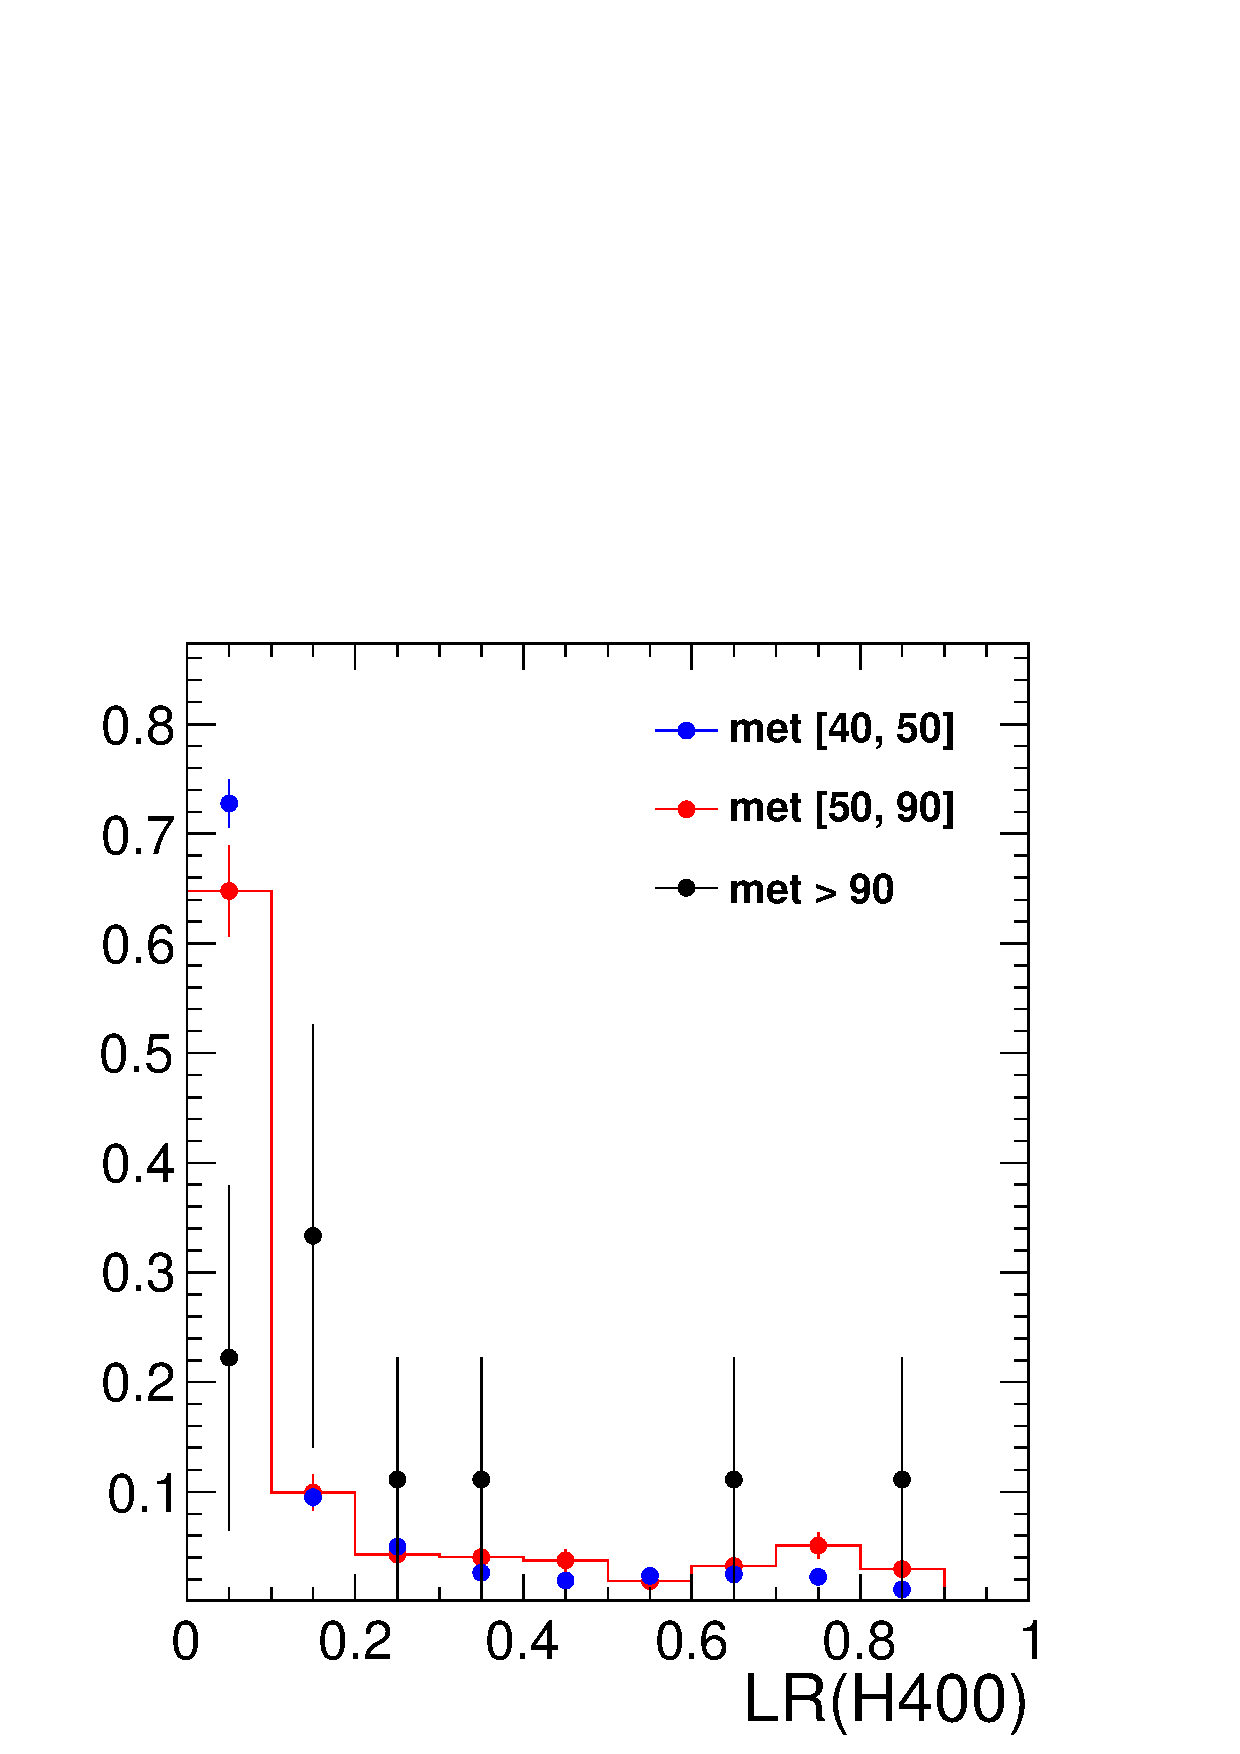
\includegraphics[width=.30\textwidth]{figures/Zmm_LR_mH400_lin.png}} 
\caption{Shape comparison of the matrix element output LR distribution in three \met regions for $Z$+jet Monte Carlo events, separately for $ee$ (left) and $\mu\mu$ (right) events. $m_H$~=~250, 300, 350 and 400 \GeVcc signal hypotheses are shown. The shapes are consistent within the uncertainties.}
\label{fig:LRshapeMET}                                                                                          
\end{figure}

\begin{figure}[!hbtp]                                                                                         
\centering  
\subfigure[]{                                                                                                 
\centering                                                                                                    
\label{subfig:lr_met250_datamc}
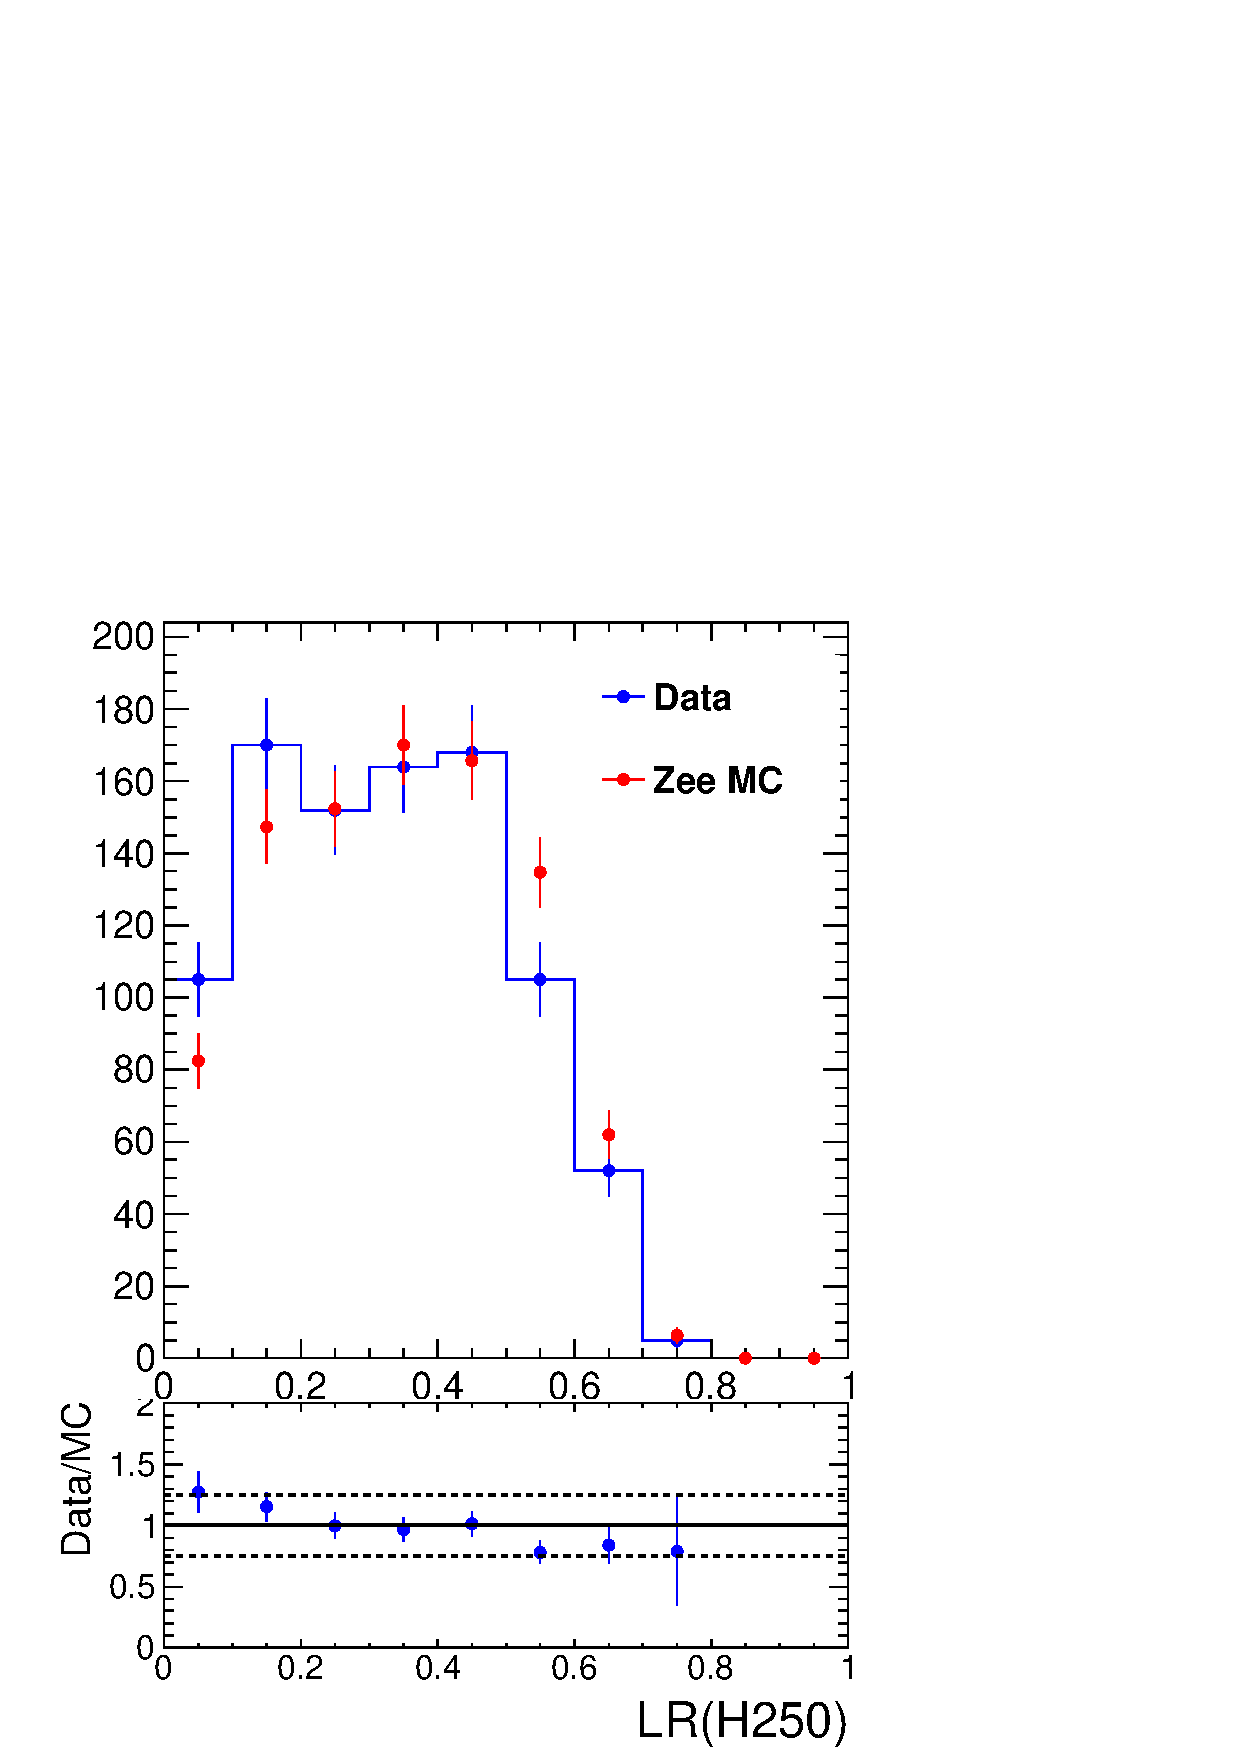
\includegraphics[width=.25\textwidth]{figures/Zee_LR_mH250_datamc_lin.png}         
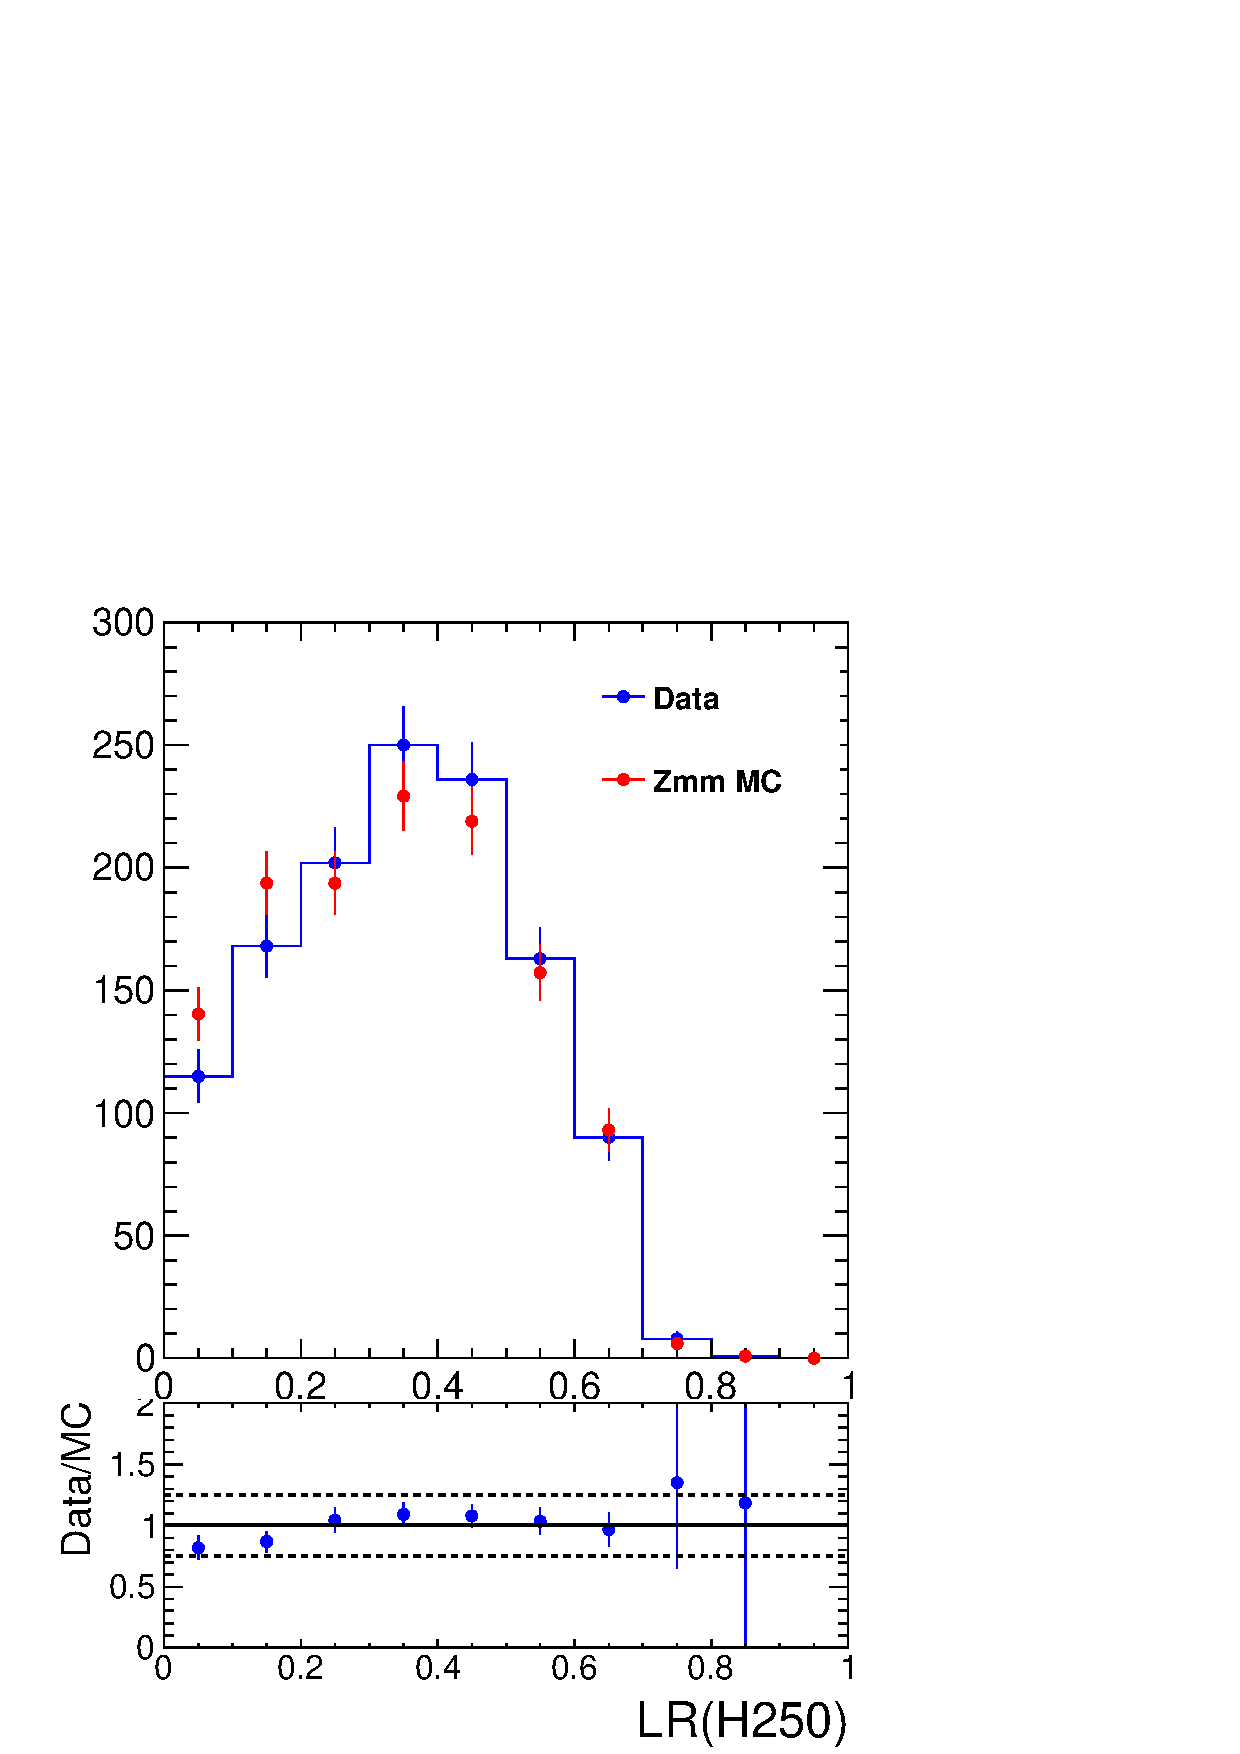
\includegraphics[width=.25\textwidth]{figures/Zmm_LR_mH250_datamc_lin.png}} 
\subfigure[]{                                                                                                 
\centering                                                                                                    
\label{subfig:lr_met300_datamc}
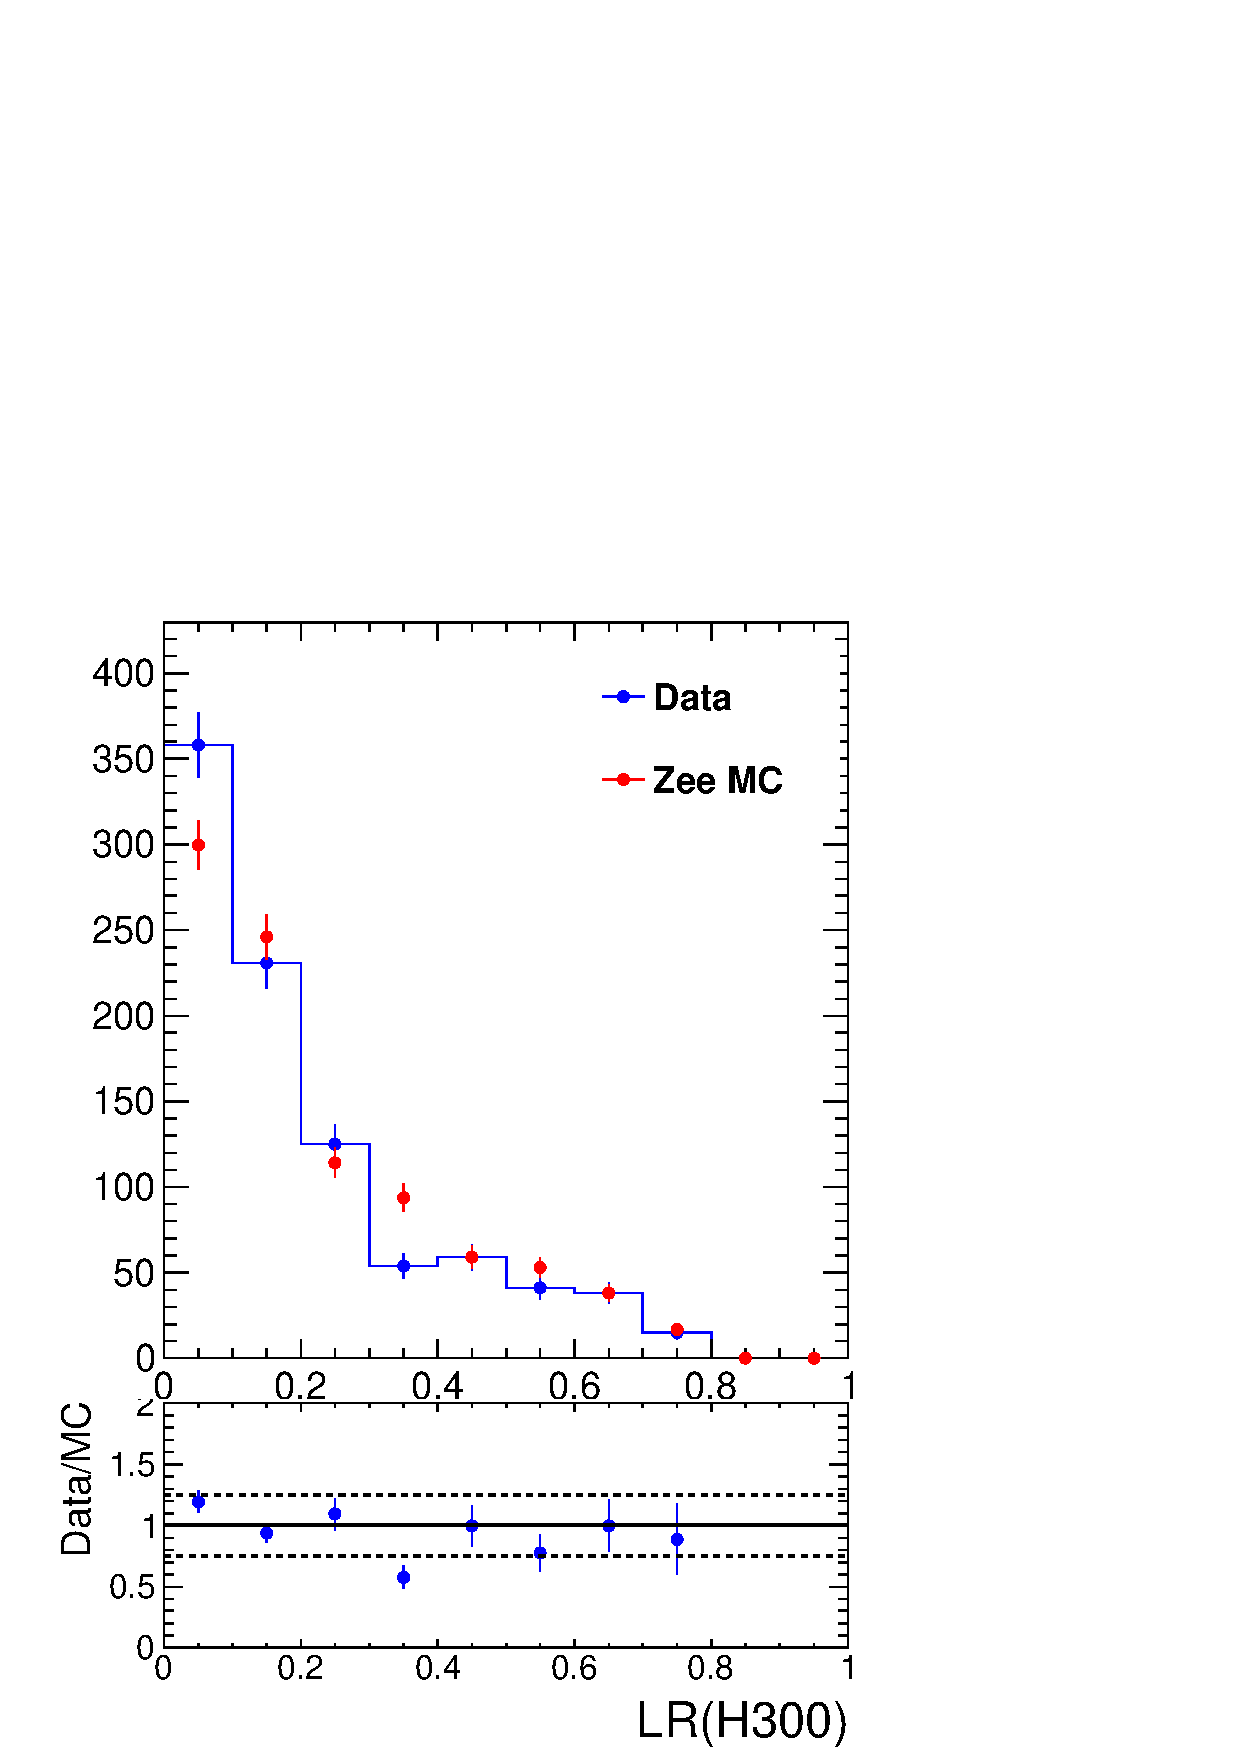
\includegraphics[width=.25\textwidth]{figures/Zee_LR_mH300_datamc_lin.png}         
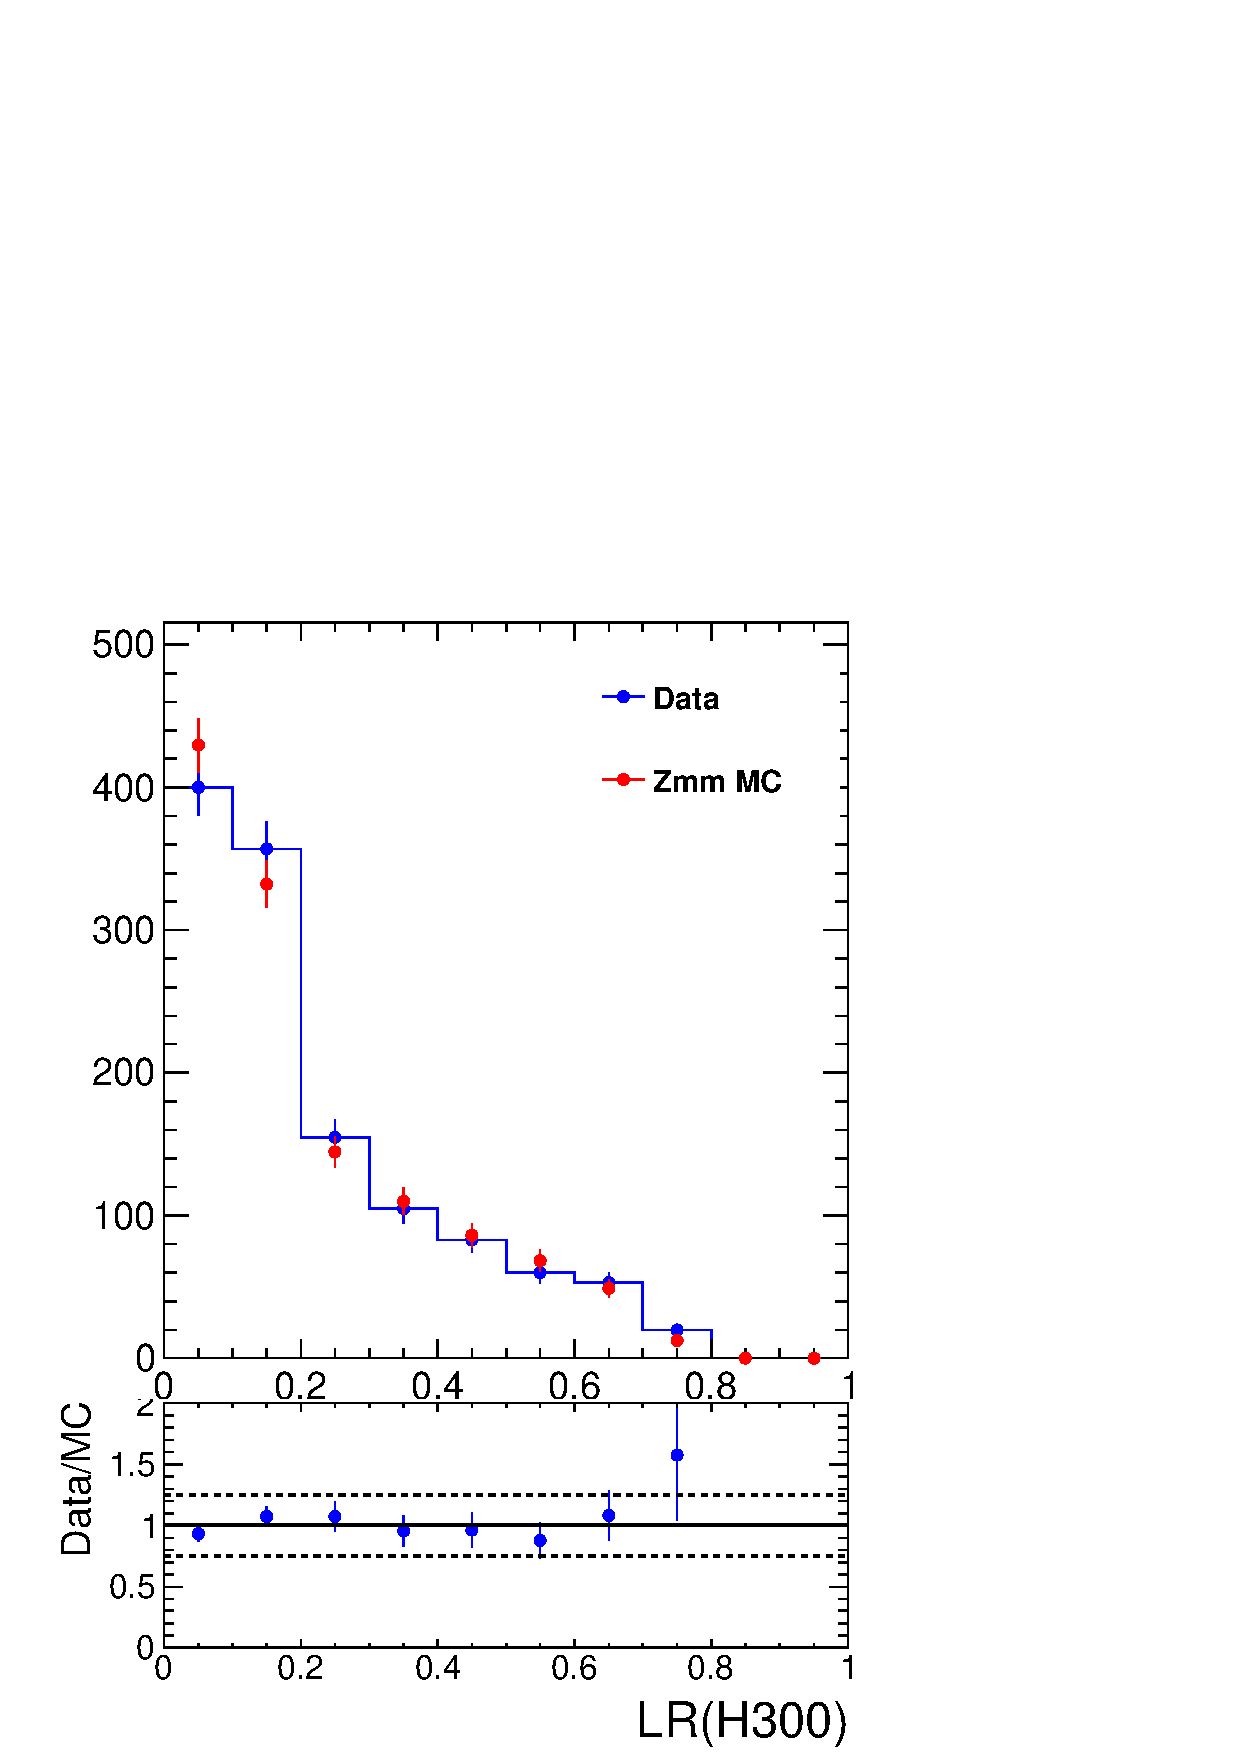
\includegraphics[width=.25\textwidth]{figures/Zmm_LR_mH300_datamc_lin.png}} 
\subfigure[]{                                                                                                 
\centering                                                                                                    
\label{subfig:lr_met350_datamc}
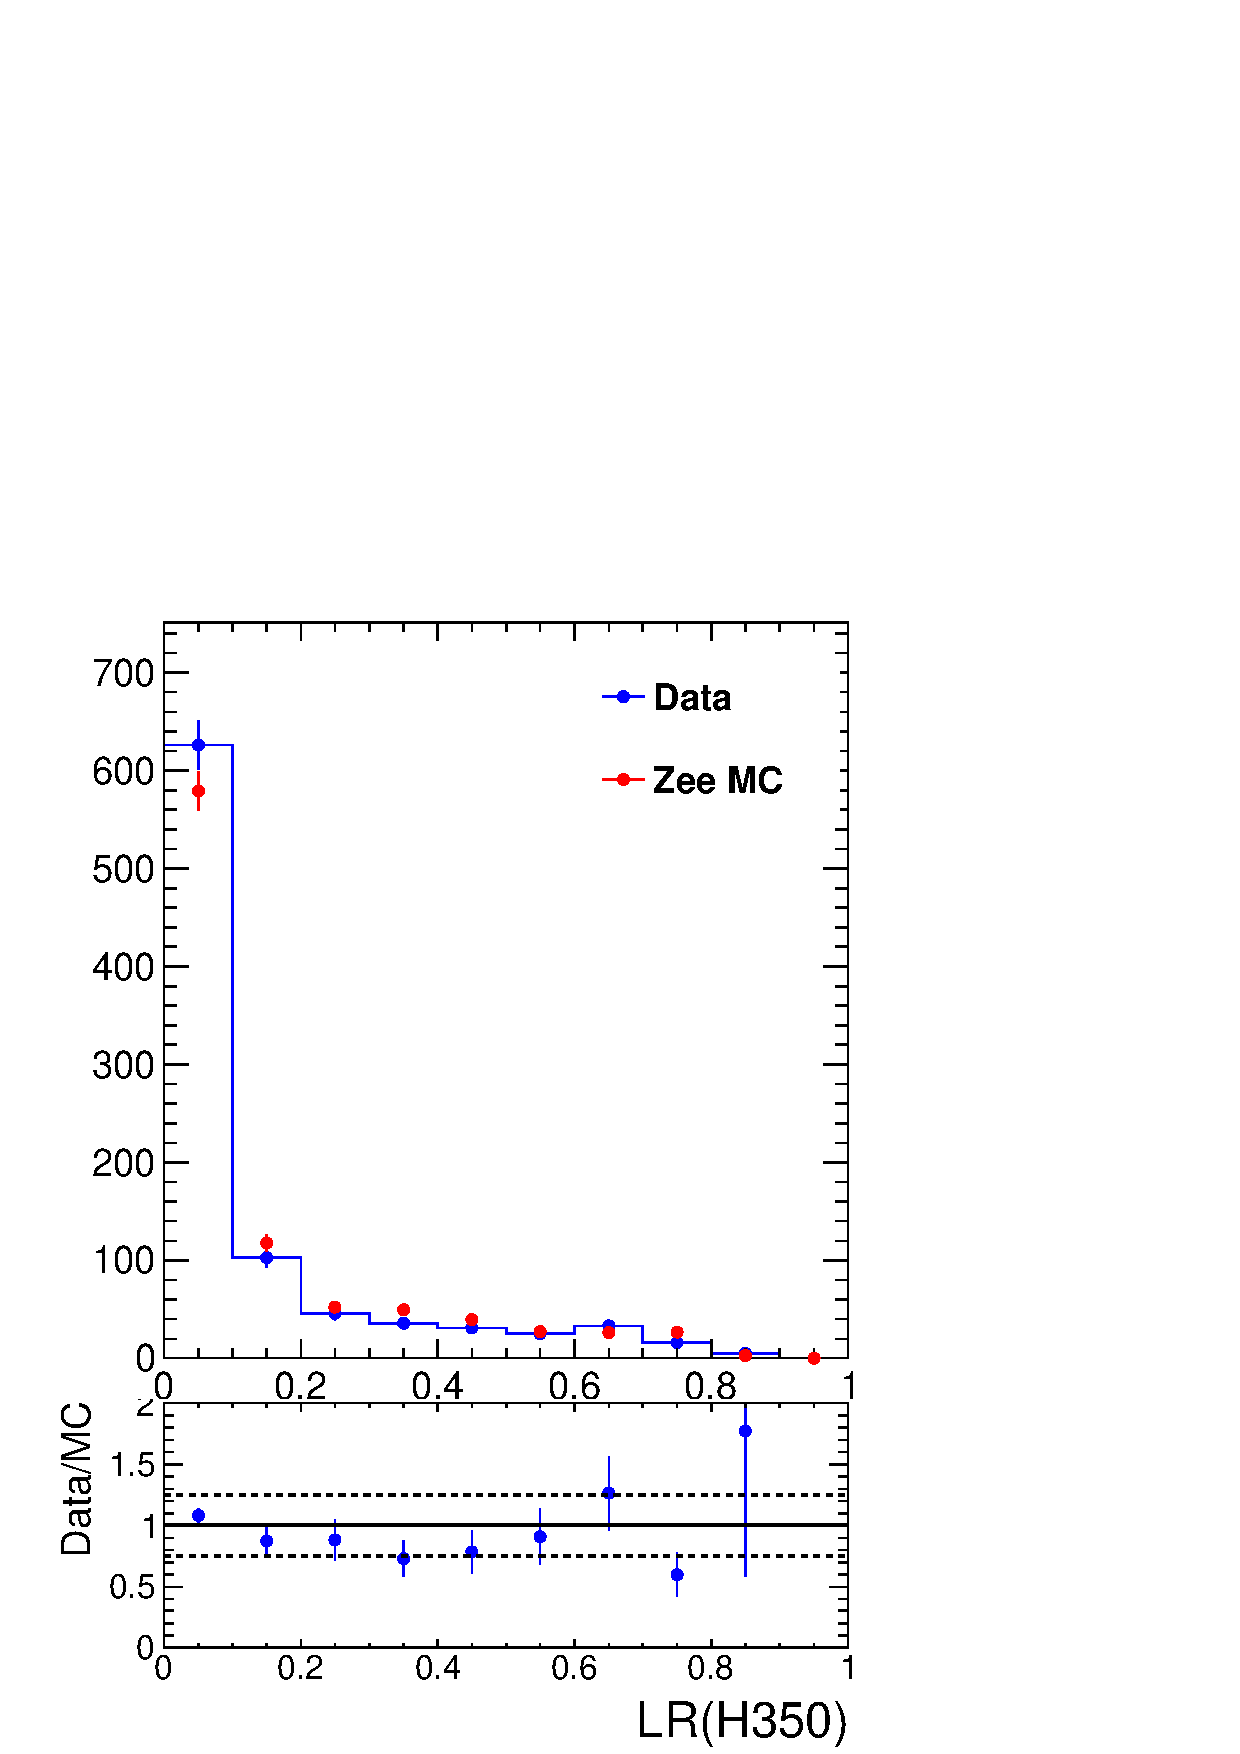
\includegraphics[width=.25\textwidth]{figures/Zee_LR_mH350_datamc_lin.png}         
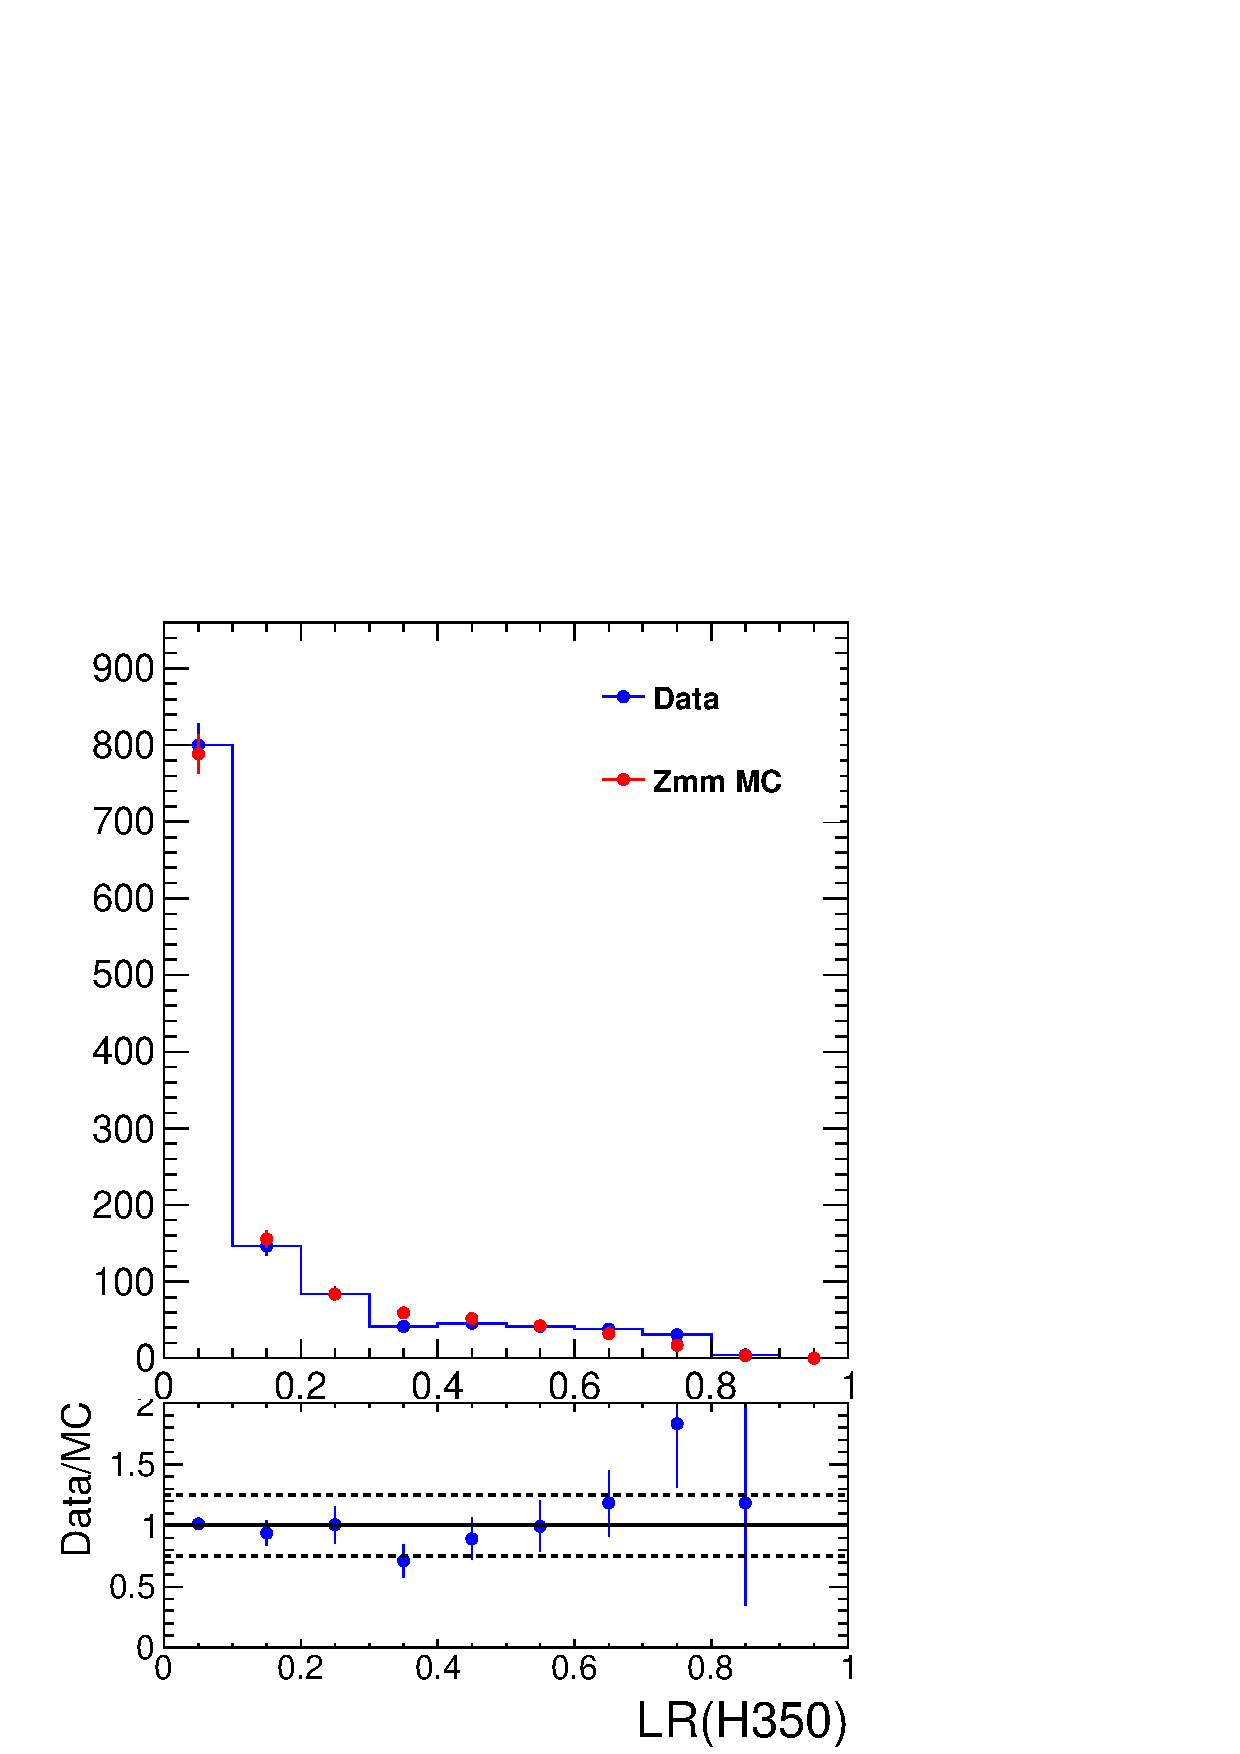
\includegraphics[width=.25\textwidth]{figures/Zmm_LR_mH350_datamc_lin.png}} 
\subfigure[]{                                                                                                 
\centering                                                                                                    
\label{subfig:lr_met400_datamc}
\includegraphics[width=.25\textwidth]{figures/Zee_LR_mH400_datamc_lin.png}         
\includegraphics[width=.25\textwidth]{figures/Zmm_LR_mH400_datamc_lin.png}} 
\caption{Shape comparison of the matrix element output LR distribution in data and MC in $40<\met<50$ GeV region, separately for $ee$ (left) and $\mu\mu$ (right) events. $m_H$~=~250, 300, 350 and 400 \GeVcc signal hypotheses are shown. The shapes are consistent within the uncertainties.}
\label{fig:LRshapeMETDataMC}                                                                                          
\end{figure}
